\documentclass[border = 1cm, preview, varwidth=\maxdimen]{standalone}

\usepackage{xeCJK}

% mathematics
\usepackage{amsmath}

% tikz
\usepackage{tikz}
\usepackage{ifthen}
\usetikzlibrary{arrows}
\usetikzlibrary{automata}
\usetikzlibrary{positioning}
\tikzset{->, > = stealth', node distance = 1in}

\begin{document}

\begin{figure}
  \centering
  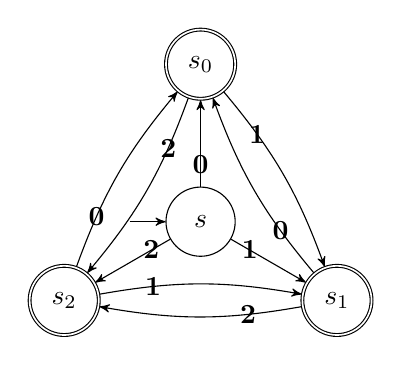
\begin{tikzpicture}
    \pgfmathtruncatemacro \digits { 3 };
    \pgfmathsetmacro \angle { 360 / \digits };
    \pgfmathtruncatemacro \n { \digits - 1 };
    % nodes
    \foreach \k in {0, ..., \n} {
      \pgfmathsetmacro \radius { 90 - \k * \angle };
      \node [state, accepting] (s\k) at (\radius:2) {$s_\k$};
    }
    \node [state, initial, initial text = ] (s) {$s$};
    % paths
    \foreach \i in {0, ..., \n} {
      \draw (s) edge [near start] node {\textbf\i} (s\i);
      \foreach \j in {0, ..., \n} {
        \ifthenelse {\i = \j}
          {}
          {\draw (s\i) edge [bend left = 10, near start] node {\textbf\j} (s\j);}
      }
    }
  \end{tikzpicture}
  \caption{状态图}
\end{figure}

\begin{figure}
  \centering
  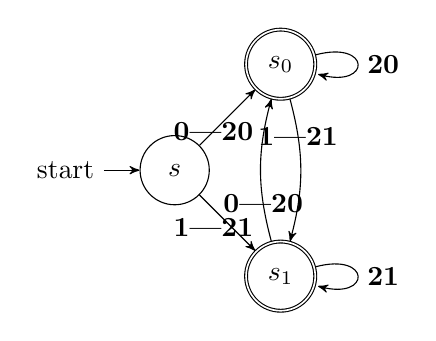
\begin{tikzpicture}
    \node [state, initial] (s) {$s$};
    \node [state, accepting, above right = 1 of s] (s0) {$s_{0}$};
    \node [state, accepting, below right = 1 of s] (s1) {$s_{1}$};
    % paths
    \draw (s) edge [near start] node {\textbf{0|20}} (s0);
    \draw (s) edge [below, near start] node {\textbf{1|21}} (s1);
    \draw (s0) edge [loop right] node {\textbf{20}} (s0);
    \draw (s1) edge [loop right] node {\textbf{21}} (s1);
    \draw (s0) edge [bend left = 15, near start] node {\textbf{1|21}} (s1);
    \draw (s1) edge [bend left = 15, near start] node {\textbf{0|20}} (s0);
  \end{tikzpicture}
  \caption{状态图(删状态 $s_2$)}
\end{figure}

\begin{figure}
  \centering
  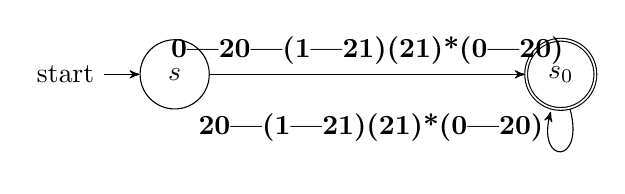
\begin{tikzpicture}
    \node [state, initial] (s) {$s$};
    \node [state, accepting, right = 4 of s] (s0) {$s_0$};
    % paths
    \draw (s) edge [above] node {\textbf{0|20|(1|21)(21)*(0|20)}} (s0);
    \draw (s0) edge [loop below, anchor = south east] node {\textbf{20|(1|21)(21)*(0|20)}\;} (s0);
  \end{tikzpicture}
  \caption{状态图(删状态 $s_1$、$s_2$)}
\end{figure}

\end{document}
